% !TEX root = ../main.tex
\documentclass[../main.tex]{subfiles}
\begin{document}

\section{Описание аппаратной части разработанной системы}

Разаботанная аппаратная часть должна отвечать следующим условиям. Прием сигнала стетоскопом осуществляется через микрофон. Далее, сигнал с микрофона должен подаваться на усилитель, усиливающий сигнал с микрофона до значений, в которых работает аналого цифровой преобразователь. Аналого цифровой преобразователь принимает сигнал и подключается к компьютеру через USB порт для передачи данных. Врач должен иметь возможность прослушивать пациента, видеть визуализацию сигнала на компьютере. Также врач должен иметь возможность увидеть спектр сигнала после преобразования Фурье.

С аппаратной точки зрения, устройство представляет собой микроконтроллер Arduino Due с подключенными к нему:
\begin{itemize}
\item микрофоном
\item усилитель
\item 2 датчика bmp280 (измерение давления чтобы детектировать вдохи и выдохи)
\item USB динамики
\end{itemize}

\begin{figure}[H]
\centering
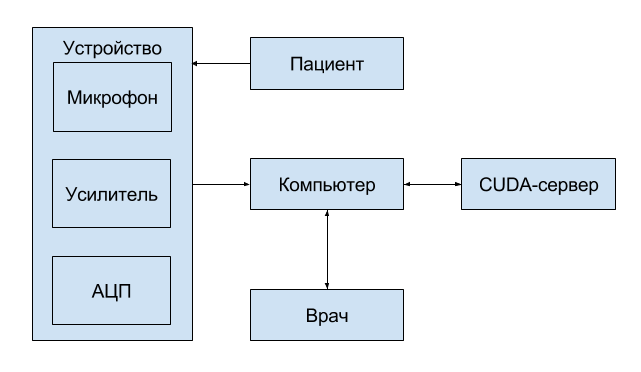
\includegraphics[width=\textwidth]{images/blueprint.png}
\caption{Схема програмно-аппаратной системы}
\end{figure}

\begin{figure}[H]
\centering
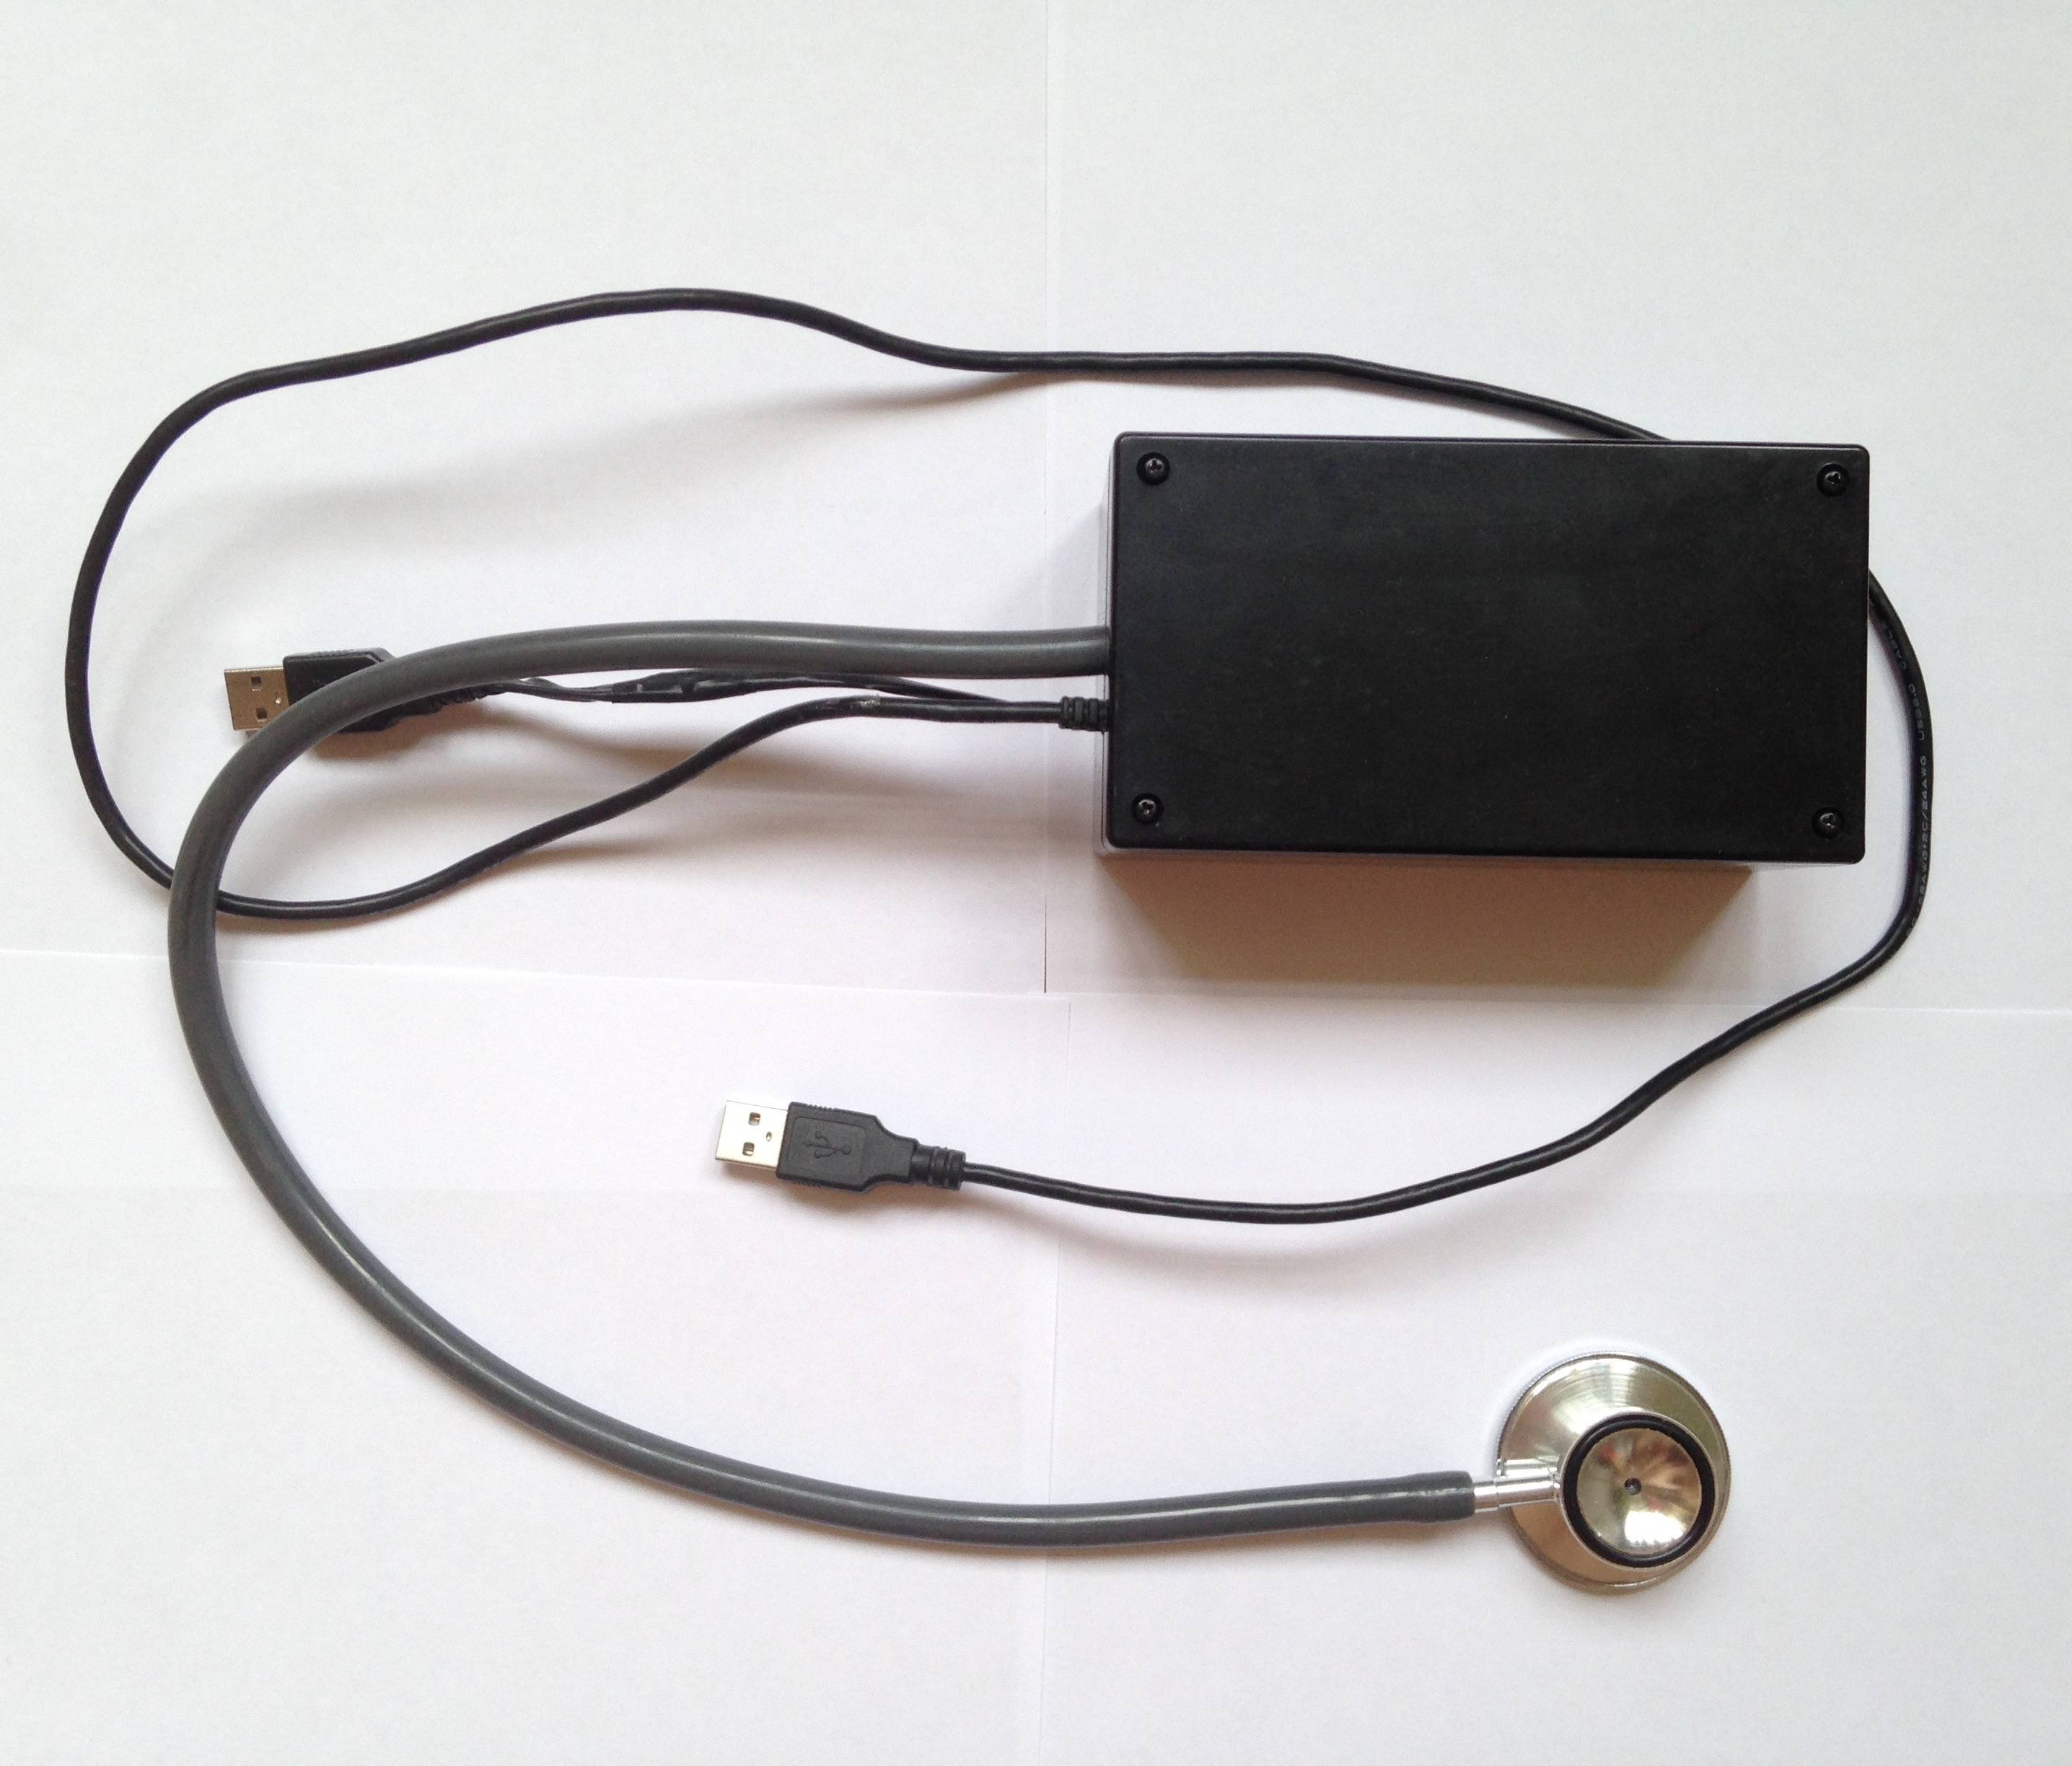
\includegraphics[width=15cm]{images/hardware.jpg}
\caption{Собранный прототип}
\end{figure}

\subsection{Описание микрофона}
В качестве микрофона был выбран SWEN MK-200. Микрофон был вынут из стандартного корпуса, чтобы лучше соединиться с трубкой, ведущей к мембране. \\

\begin{table}[h]
\centering
\caption{Технические характеристики SWEN MK-200}
\begin{tabular}{|l|l|}
\hline
Чувствительность, дБ           & -60 ± 3                    \\ \hline
Диапазон частот, Гц            & 50 – 16 000                \\ \hline
Размер микрофонного модуля, мм & 9×7                        \\ \hline
Тип разъема                    & мини-джек Ø 3,5 мм (3 pin) \\ \hline
Длина кабеля, м                & 1,8                        \\ \hline
Вес, г                         & 63                         \\ \hline
\end{tabular}
\end{table}

Наилучшая чувствительность данного микрофона достигается в диапазоне частот от 50 до 16000 Гц. Тем не менее, микрофон с ослаблением принимает сигнал вплоть до 40кГц. Поэтому данный микрофон подходит для данного проекта.

Для подавления шумов и лучшей передачи звука от сердца, легких и других органов к микрофону присоединяются мембрана и соединительная трубка от аналогового стетоскопа.

\subsection{Описание усилителя}
Усилитель для микрофона был создан самостоятельно в рамках данной работы на базе операционного усилителя \textbf{MCP6022} от производителя Microchip. Это усилитель типа Rail-to-Rail SO-8. Была выбрана следующая схема усилителя:

\begin{figure}[H]
\centering
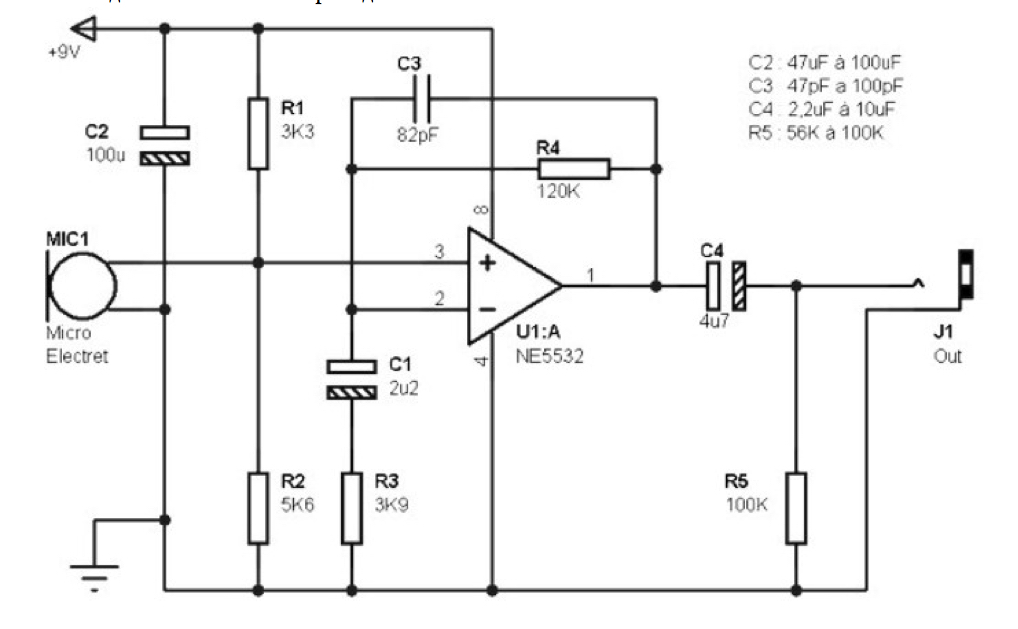
\includegraphics[width=14cm]{images/circuit.jpg}
\caption{Схема усилителя сигнала}
\end{figure}

\subsection{Микроконтроллер Arduino Due}
Самым оптимальным вариантом микроконтроллера для данного проекта оказался Arduino Due. Он сочетает в себе как простоту в использовании так и возможность оцифровывать сигнал высокого качества. Максимальная частота дискретизации АЦП Arduino Due составляет 1МГЦ. В ходе данной работы удалось достичь максимума в 700кГц. Обычно среднее значение частоты дискретизации составляло 670кГц. Максимальное значение частоты дискретизации зависит также от производительности компьютера. Данное устройство тестировалось на MacBook Air 2014.

\begin{figure}[H]
\centering
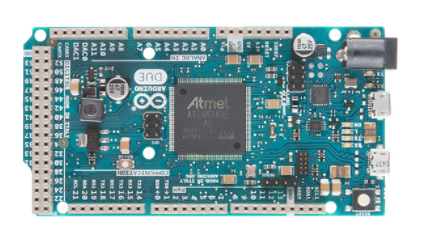
\includegraphics[width=10cm]{images/adc3}
\caption{Микроконтроллер Arduino Due}
\end{figure}

\begin{table}[H]
\centering
\caption{Технические характеристики Arduino Due}

\begin{tabular}{|l|l|}
                                                                      \hline
Число аналоговых входов            & 12                            \\ \hline
Максимальная частота дискретизации & 1МГц                          \\ \hline
Объем буффера памяти               & 512 KB					               \\ \hline
Разрядность                        & 12бит (4096 значений)         \\ \hline
Рабочее напряжение                 & 3.3V                          \\ \hline
Диапазоны входного напряжения      & 7-12V                         \\ \hline
Защита по входному напряжению      & 6-16V                         \\ \hline
Интерфейс                          & USB                           \\ \hline
Микроконтроллер                    & AT91SAM3X8E                   \\ \hline
Масса                              & 36г                           \\ \hline
\end{tabular}
\end{table}

\newpage
\end{document}
